\documentclass[11pt]{article}
\usepackage[T1]{fontenc}
\usepackage[utf8]{inputenc}
\usepackage[spanish]{babel}
\usepackage{amsmath,amssymb}
\usepackage[a4paper,margin=2.3cm]{geometry}
\usepackage{graphicx}
\usepackage{float}
\usepackage[inkscapelatex=false]{svg}
\usepackage{tikz}
\usetikzlibrary{arrows.meta,patterns,babel}
\usepackage{hyperref}
\hypersetup{hidelinks}
\spanishdecimal{.}
% Evita que las abreviaturas de babel interfieran con las flechas TikZ.
\AtBeginDocument{\shorthandoff{<>}}
\setlength{\parindent}{0pt}
\setlength{\parskip}{0.4em}
\setlength{\abovedisplayskip}{6pt}
\setlength{\belowdisplayskip}{6pt}
\providecommand{\graficanumerica}[2][]{\includesvg[#1]{figuras/#2}}
\newcommand{\encabezado}[1]{%
  {\Large\bfseries #1\par}\vspace{3pt}
  {\normalsize Electrodinámica I\hfill P.S., J.A., J.R.\par}
  \vspace{6pt}\hrule\vspace{8pt}}
\newcommand{\er}{\hat{\mathbf r}}
\newcommand{\normal}{\hat{\mathbf n}}
\newcommand{\dd}{\,\mathrm d}
\tikzset{>=Stealth,line cap=round,line join=round,
  every node/.style={font=\small},
  gaussiana/.style={densely dashed,line width=0.9pt},
  vector/.style={-{Stealth[length=2mm]},line width=0.9pt}}

\begin{document}
\encabezado{Desplazamiento eléctrico y ley de Gauss}


% Enunciado y figura del sistema.
Una carga puntual libre $q$ se encuentra en el origen ($r=0$). Concéntrica
con ella, se dispone una capa esférica de material dieléctrico lineal,
homogéneo e isotrópico, de permitividad relativa $\varepsilon_r$ y
permitividad $\varepsilon=\varepsilon_0\varepsilon_r$. El material ocupa
$R_1<r<R_2$, con $0<R_1<R_2$; la cavidad y el exterior están en el vacío.
El sistema se representa en la figura~\ref{fig:sistema}.

Determine analíticamente en las tres regiones:
\begin{enumerate}
  \item El desplazamiento eléctrico $\vec D$.
  \item El campo eléctrico $\vec E$.
  \item La polarización $\vec P$.
  \item La densidad volumétrica de carga ligada $\rho_b$ en el material
  y las densidades superficiales $\sigma_b$ en $r=R_1$ y $r=R_2$.
  Compruebe que la carga ligada total del sistema es cero.
  \item Discuta y demuestre qué ocurre cuando el material se vuelve
  idéntico al vacío ($\varepsilon_r\to1$) y en el límite
  $\varepsilon_r\to\infty$, que se comparará con un conductor perfecto.
\end{enumerate}

\begin{figure}[H]
\centering

% (a) Vista tridimensional
\begin{minipage}[c]{0.49\textwidth}
\centering
\resizebox{0.60\linewidth}{!}{%
\begin{tikzpicture}[line join=round,line cap=round]
  % Ambas vistas tienen el mismo encuadre y radio exterior.
  \path[use as bounding box] (-2.9,-3.1) rectangle (3.2,3.1);

  % Proyección ortográfica isométrica.
  % Se retira el octante x,y,z>0 para mostrar el interior.
  \def\Rext{2.30}
  \def\Rint{1.12}

  \shade[ball color=black!26]
    (0,0) circle[radius=\Rext cm];
  \draw[black!70,thick]
    (0,0) circle[radius=\Rext cm];

  % Cavidad.
  \shade[inner color=white,outer color=black!18]
    (0,0) circle[radius=\Rint cm];

  \begin{scope}[
    x={(0.707107cm,-0.408248cm)},
    y={(-0.707107cm,-0.408248cm)},
    z={(0cm,0.816497cm)}
  ]
    % Caras anulares del corte.
    \path[fill=black!31]
      plot[domain=0:90,samples=65,variable=\t]
        ({\Rext*cos(\t)},{\Rext*sin(\t)},0)
      -- plot[domain=90:0,samples=65,variable=\t]
        ({\Rint*cos(\t)},{\Rint*sin(\t)},0)
      -- cycle;

    \path[fill=black!16]
      plot[domain=0:90,samples=65,variable=\t]
        ({\Rext*cos(\t)},0,{\Rext*sin(\t)})
      -- plot[domain=90:0,samples=65,variable=\t]
        ({\Rint*cos(\t)},0,{\Rint*sin(\t)})
      -- cycle;

    \path[
      fill=black!8,
      postaction={
        pattern=north east lines,
        pattern color=black!25
      }
    ]
      plot[domain=0:90,samples=65,variable=\t]
        (0,{\Rext*cos(\t)},{\Rext*sin(\t)})
      -- plot[domain=90:0,samples=65,variable=\t]
        (0,{\Rint*cos(\t)},{\Rint*sin(\t)})
      -- cycle;

    % Fronteras de las superficies de corte.
    \foreach \rr in {\Rint,\Rext} {
      \draw[thick]
        plot[domain=0:90,samples=65,variable=\t]
          ({\rr*cos(\t)},{\rr*sin(\t)},0);

      \draw[thick]
        plot[domain=0:90,samples=65,variable=\t]
          ({\rr*cos(\t)},0,{\rr*sin(\t)});

      \draw[thick]
        plot[domain=0:90,samples=65,variable=\t]
          (0,{\rr*cos(\t)},{\rr*sin(\t)});
    }

    % Aristas radiales.
    \draw[thick] (\Rint,0,0)--(\Rext,0,0);
    \draw[thick] (0,\Rint,0)--(0,\Rext,0);
    \draw[thick] (0,0,\Rint)--(0,0,\Rext);

    % Radios.
    \draw[vector] (0,0,0)--(0,0,\Rint);
    \draw[vector] (0,0,0)--(\Rext,0,0);
  \end{scope}

  % Carga central y etiquetas.
  \fill (0,0) circle (2.5pt);
  \node[below left=3pt] at (0,0) {$q$};
  \node at (-0.27,0.55) {$R_1$};
  \node at (0.91,-0.84) {$R_2$};
\end{tikzpicture}%
}

\par\smallskip
{\small (a) Vista tridimensional}
\end{minipage}\hfill
%
% (b) Corte transversal xy
\begin{minipage}[c]{0.49\textwidth}
\centering
\resizebox{0.60\linewidth}{!}{%
\begin{tikzpicture}[line join=round,line cap=round]
  \path[use as bounding box] (-2.9,-3.1) rectangle (3.2,3.1);

  % Corte central en el plano xy.
  \fill[
    pattern=north east lines,
    pattern color=black!40,
    even odd rule
  ]
    (0,0) circle (2.30)
    (0,0) circle (1.12);

  \draw[thick] (0,0) circle (2.30);
  \draw[thick] (0,0) circle (1.12);

  % Ejes del corte.
  \draw[->,thin]
    (-2.75,0)--(2.85,0)
    node[below=2pt] {$x$};

  \draw[->,thin]
    (0,-2.55)--(0,2.7)
    node[above] {$y$};

  % Radios.
  \draw[vector] (0,0)--(140:1.12);
  \node at (-0.52,0.16) {$R_1$};

  \draw[vector]
    (0,0)--(-38:2.30)
    node[pos=0.74,above right] {$R_2$};

  % Carga central.
  \fill (0,0) circle (2.2pt);
  \node[below right=3pt] at (0,0) {$q$};
\end{tikzpicture}%
}

\par\smallskip
{\small (b) Corte transversal $xy$}
\end{minipage}

% Leyenda común a las dos vistas.
\par\medskip
{\small
\begin{tabular}{
  @{}c@{\hspace{0.8cm}}
  c@{\hspace{0.8cm}}
  c@{}
}
  I. Cavidad: vacío
  & II. Dieléctrico
  & III. Exterior: vacío
  \\[2pt]
  $0<r<R_1$
  & $R_1<r<R_2$
  & $r>R_2$
  \\[2pt]
  $\varepsilon=\varepsilon_0$
  & $\varepsilon=\varepsilon_0\varepsilon_r$
  & $\varepsilon=\varepsilon_0$
\end{tabular}
\par
}

\caption{(a) Vista tridimensional del cascarón esférico con un octante
retirado para mostrar su interior. La zona gris es el dieléctrico;
la cavidad contiene vacío y una carga puntual en su centro.
(b) Corte transversal de la esfera. Se representa la carga puntual
en el centro y se observan las tres regiones del sistema.
La zona rayada corresponde al dieléctrico. En ambas vistas se indican
los intervalos de la coordenada radial $r$ y la permitividad
dieléctrica correspondiente a cada región (cavidad vacía, dieléctrico
y exterior en el vacío).}
\label{fig:cascaron3d}
\label{fig:sistema}
\end{figure}

\newpage

\section*{Solución}
Usamos coordenadas esféricas $(r,\theta,\varphi)$ con origen $O$ en la
carga (figura~\ref{fig:coordenadas}). La carga puntual $q$ está fija en
$\vec x'=\vec0$, y el punto de observación $P$ se localiza mediante
$\vec x=r\er$, donde $r=|\vec x|\in(0,\infty)$ es la coordenada radial.
El ángulo colatitudinal $\theta\in[0,\pi]$ se mide desde el semieje
$+z$ hasta $\vec x$, mientras que el azimutal $\varphi\in[0,2\pi)$
se mide desde $+x$ hacia $+y$ en el plano $xy$. Dado que el dieléctrico
es homogéneo e isótropo\footnote{Un material es homogéneo si sus propiedades no dependen de la posición (son las mismas en todo el material); es isótropo si sus propiedades no dependen de la dirección. La homogeneidad compara puntos distintos; la isotropía, direcciones distintas en un mismo punto. En este problema, la isotropía implica que la permitividad es la misma en todas las direcciones.} y las fronteras son esféricas y
concéntricas con la carga, el sistema tiene simetría esférica.
Por consiguiente, los campos físicos son radiales y sus componentes
solo dependen de $r$.

\begin{figure}[H]
\centering
\resizebox{0.40\textwidth}{!}{%
\begin{tikzpicture}[line cap=round,line join=round]
  % Proyección ortográfica: cámara en la dirección (1,1,0.8).
  % +x baja hacia la izquierda; +y baja hacia la derecha; +z sube.
  \def\Rext{2.30}
  \def\Rint{1.12}
  \def\radio{2.05}
  \def\polar{50}
  \def\azimut{110}

  \path[use as bounding box]
    (-3.0,-2.55) rectangle (3.0,3.15);

  % Coordenadas cartesianas del punto de observación.
  \pgfmathsetmacro{\px}{\radio*sin(\polar)*cos(\azimut)}
  \pgfmathsetmacro{\py}{\radio*sin(\polar)*sin(\azimut)}
  \pgfmathsetmacro{\pz}{\radio*cos(\polar)}

  % Superficies esféricas transparentes.
  \draw[black!35]
    (0,0) circle[radius=\Rext cm];
  \draw[black!20,densely dashed]
    (0,0) circle[radius=\Rint cm];

  \begin{scope}[
    x={(-0.707107cm,-0.348155cm)},
    y={(0.707107cm,-0.348155cm)},
    z={(0cm,0.870388cm)}
  ]
    % Circunferencia en el plano xy.
    \draw[black!25,densely dashed]
      plot[domain=0:360,samples=121,variable=\t]
        ({\Rext*cos(\t)},{\Rext*sin(\t)},0);

    % Ejes cartesianos.
    \draw[->,thin]
      (0,0,0)--(3.12,0,0)
      node[below left] {$x$};

    \draw[->,thin]
      (0,0,0)--(0,3.12,0)
      node[below right] {$y$};

    \draw[->,thin]
      (0,0,0)--(0,0,3.12)
      node[above] {$z$};

    % Punto de observación y proyección sobre el plano xy.
    \coordinate (P) at (\px,\py,\pz);
    \coordinate (H) at (\px,\py,0);

    \draw[densely dashed,black!65]
      (0,0,0)--(H)--(P);

    \fill[black!65] (H) circle (1.3pt);

    % Vector posición del punto de observación.
    \draw[vector,line width=1.1pt]
      (0,0,0)--(P)
      node[pos=0.68,above left=2pt] {$\vec x$};

    \fill (P) circle (2pt);
    \node[above right=3pt] at (P) {$P$};

    % Ángulo colatitudinal.
    \draw[->,line width=0.8pt]
      plot[domain=0:\polar,samples=41,variable=\t]
        ({0.95*sin(\t)*cos(\azimut)},
         {0.95*sin(\t)*sin(\azimut)},
         {0.95*cos(\t)});

    % Ángulo azimutal.
    \draw[->,line width=0.8pt]
      plot[domain=0:\azimut,samples=41,variable=\t]
        ({1.00*cos(\t)},{1.00*sin(\t)},0);
  \end{scope}

  % Origen y etiquetas angulares.
  \fill (0,0) circle (2.5pt);
  \node[above left=4pt] at (0,0) {$O$};
  \node at (0.22,0.70) {$\theta$};
  \node at (-0.08,-0.75) {$\varphi$};
\end{tikzpicture}%
}

\caption{Sistema de referencia esférico y posiciones de la carga puntual
y del punto de observación.}
\label{fig:coordenadas}
\end{figure}

\subsection*{1. Desplazamiento eléctrico}
Sabemos que una carga puntual $q$ en reposo, respecto de un sistema
de referencia inercial, es de por sí una fuente de campo eléctrico,
con una singularidad en la posición de la carga. El campo eléctrico
de esta carga aislada en el vacío se extiende por todo el espacio,
y su magnitud decrece con el inverso del cuadrado de la distancia
a la fuente. En particular, cuando el campo eléctrico del sistema
actúa sobre la región del medio dieléctrico lineal,
$r\in(R_1,R_2)$, redistribuye las cargas de las moléculas que
conforman el material, de modo que podemos describir esta
redistribución en términos de cargas ligadas
(figura~\ref{fig:polarizacion}).

\begin{figure}
\centering
\resizebox{0.72\textwidth}{!}{%
\begin{tikzpicture}[
  scale=0.95,
  carga/.style={
    circle,
    draw=black,
    fill=white,
    line width=0.5pt,
    inner sep=0pt,
    minimum size=3.4mm,
    font=\small
  }
]
  % Corte transversal del cascarón dieléctrico.
  \fill[black!12,even odd rule]
    (0,0) circle (2.05)
    (0,0) circle (1.10);

  \draw[thick] (0,0) circle (2.05);
  \draw[thick] (0,0) circle (1.10);

  % Polarización radial dentro del material.
  \foreach \ang in {0,60,...,300} {
    \draw[vector] (\ang:1.40)--(\ang:1.77);
  }

  % Cargas ligadas superficiales, dibujadas del lado del dieléctrico.
  % Los símbolos representan distribuciones superficiales continuas.
  \foreach \ang in {15,45,...,345} {
    \node[carga] at (\ang:1.28) {$-$};
    \node[carga] at (\ang:1.87) {$+$};
  }

  % Carga libre central.
  \fill (0,0) circle (2pt);
  \node at (0,-0.35) {$q$};

  % Normales que salen del dieléctrico.
  \draw[vector,very thick]
    (150:1.10)--(150:0.48);
  \node at (-0.48,0.72) {$\normal_1$};

  \draw[vector,very thick]
    (25:2.05)--(25:2.82);
  \node[above right] at (25:2.65) {$\normal_2$};

  \node at (0,-2.52)
    {$\normal_1=-\er,\qquad\normal_2=+\er$};

  \node at (0,-3.02)
    {$\vec P=P_r\er$ en el material};

  % Esquema de dipolos alineados.
  % Esquema de dipolos alineados.
  \begin{scope}[
    xshift=3.5cm,
    carga dipolo/.style={
      circle,
      draw=black,
      fill=white,
      line width=0.5pt,
      inner sep=0pt,
      outer sep=0pt,
      minimum size=3.6mm,
      font=\small
    }
  ]
    \node at (3.25,1.75) {Fila de dipolos alineados};

    % Cuatro dipolos separados.
    % Los signos van dentro de los círculos, no debajo.
    \foreach \xx in {0,1.05,2.10,3.15} {
      \draw[thin]
        (\xx,0.65)--({\xx+0.55},0.65);

      \node[carga dipolo]
        at (\xx,0.65) {$\boldsymbol{-}$};

      \node[carga dipolo]
        at ({\xx+0.55},0.65) {$\boldsymbol{+}$};
    }

    % Representación macroscópica.
    \node[font=\large] at (4.20,0.65) {$\simeq$};

    \draw[thin]
      (4.75,0.65)--(6.50,0.65);

    \node[carga dipolo]
      at (4.75,0.65) {$\boldsymbol{-}$};

    \node[carga dipolo]
      at (6.50,0.65) {$\boldsymbol{+}$};

    \node[align=center] at (3.25,-0.65)
      {Promedio macroscópico:\\
       cargas en los extremos, carga neta nula.};
  \end{scope}
\end{tikzpicture}%
}
\caption{Cargas ligadas en las superficies del dieléctrico para
$q>0$: negativas en la interna y positivas en la externa.
A la derecha, compensación de cargas en una fila de dipolos.}
\label{fig:polarizacion}
\end{figure}

A esta redistribución de cargas la llamamos polarización y la
describimos mediante un campo vectorial $\vec P$, que representa
el momento dipolar eléctrico por unidad de volumen. En este
problema, la polarización es no nula en la región ocupada por
el dieléctrico y nula en el resto del sistema.

Partimos de la ley de Gauss para el campo eléctrico, donde la
carga total encerrada $Q_{\mathrm{tot}}$ es la suma de la carga
libre $Q_f$ (en este contexto, la carga puntual $q$) y la carga
ligada $Q_b$, de modo que
\begin{align}
  \oint_S\vec E\cdot\dd\vec a
    &=\frac{Q_{\mathrm{tot}}}{\varepsilon_0}
      \notag\\
    &=\frac{1}{\varepsilon_0}\left(Q_f+Q_b\right).
      \label{eq:gauss_E_total}
\end{align}
Multiplicamos \eqref{eq:gauss_E_total} por la permitividad
dieléctrica del vacío $\varepsilon_0$ y obtenemos
\begin{equation}
  \varepsilon_0\oint_S\vec E\cdot\dd\vec a=Q_f+Q_b.
  \label{eq:gauss_E_libre_ligada}
\end{equation}
La carga ligada encerrada, considerando tanto las cargas de volumen
como las de superficie (véase la sección 4.2.2,
\emph{Physical Interpretation of Bound Charges}, de
\emph{Introduction to Electrodynamics}, de Griffiths), se relaciona
con la polarización mediante
\begin{equation}
  Q_b=-\oint_S\vec P\cdot\dd\vec a.
  \label{eq:Qb_flujo_P}
\end{equation}
Sustituyendo \eqref{eq:Qb_flujo_P} en
\eqref{eq:gauss_E_libre_ligada} y reagrupando las integrales,
obtenemos
\begin{align}
  \varepsilon_0\oint_S\vec E\cdot\dd\vec a
    &=Q_f-\oint_S\vec P\cdot\dd\vec a,
      \notag\\
  \varepsilon_0\oint_S\vec E\cdot\dd\vec a
    +\oint_S\vec P\cdot\dd\vec a
    &=Q_f,
      \notag\\
  \oint_S
    \bigl(\varepsilon_0\vec E+\vec P\bigr)
    \cdot\dd\vec a
    &=Q_f.
      \label{eq:gauss_D}
\end{align}
Definimos entonces el \emph{vector de desplazamiento eléctrico} como
\begin{equation}
  \vec D=\varepsilon_0\vec E+\vec P.
  \label{eq:def_D}
\end{equation}
Sustituyendo la definición \eqref{eq:def_D} en
\eqref{eq:gauss_D}, obtenemos la ley de Gauss para
el desplazamiento eléctrico:
\begin{equation}
  \oint_S\vec D\cdot\dd\vec a=Q_f.
  \label{eq:gauss_D_integral}
\end{equation}
Esta ecuación nos dice que el flujo del desplazamiento eléctrico
a través de la superficie gaussiana cerrada $S$ es igual a la
carga libre neta que esta encierra. Es decir, nos da información
sobre la carga libre encerrada, pese a la polarización del material
y a la presencia de cargas ligadas en el sistema.

Elegimos una esfera gaussiana de radio $r$ centrada en $q$
(figura~\ref{fig:gauss}). Sobre ella, $r$ es constante y el
elemento de área escalar en coordenadas esféricas es de la forma
\[
  \dd a=r^2\sin\theta\dd\theta\dd\varphi.
\]
Por su parte, el elemento de área vectorial es normal a la
superficie gaussiana, de modo que
$\dd\vec a=\dd a\,\hat{\mathbf n}$.
Como la normal unitaria exterior $\hat{\mathbf n}$ coincide
con el vector unitario radial $\er$
(figura~\ref{fig:normal_gaussiana}), obtenemos
\begin{align*}
  \dd\vec a
    &=\dd a\,\er\\
    &=r^2\sin\theta\dd\theta\dd\varphi\,\er.
\end{align*}
\begin{figure}[H]
\centering
\begin{tikzpicture}[
  line cap=round,
  line join=round,
  every node/.style={font=\small}
]
  \def\Rg{2.15}

  % Dirección radial del punto donde se dibuja el elemento de área.
  \pgfmathsetmacro{\nx}{sin(50)*cos(110)}
  \pgfmathsetmacro{\ny}{sin(50)*sin(110)}
  \pgfmathsetmacro{\nz}{cos(50)}

  % Contorno aparente de la superficie gaussiana.
  \draw[densely dashed,line width=0.9pt]
    (0,0) circle[radius=\Rg cm];

  % Proyección ortográfica del sistema tridimensional.
  \begin{scope}[
    x={(-0.707107cm,-0.348155cm)},
    y={(0.707107cm,-0.348155cm)},
    z={(0cm,0.870388cm)}
  ]
    % Circunferencia ecuatorial como ayuda para visualizar la esfera.
    \draw[black!40,densely dashed]
      plot[domain=0:360,samples=121,variable=\t]
        ({\Rg*cos(\t)},{\Rg*sin(\t)},0);

    % Punto de la superficie y extremo de la normal exterior.
    \coordinate (G) at
      ({\Rg*\nx},{\Rg*\ny},{\Rg*\nz});

    \coordinate (N) at
      ({(\Rg+0.85)*\nx},
       {(\Rg+0.85)*\ny},
       {(\Rg+0.85)*\nz});

    % Elemento curvo de área sobre la esfera r = constante.
    \path[draw=black,fill=black!20,line width=0.8pt]
      plot[domain=44:56,samples=15,variable=\t]
        ({\Rg*sin(\t)*cos(104)},
         {\Rg*sin(\t)*sin(104)},
         {\Rg*cos(\t)})
      -- plot[domain=104:116,samples=15,variable=\t]
        ({\Rg*sin(56)*cos(\t)},
         {\Rg*sin(56)*sin(\t)},
         {\Rg*cos(56)})
      -- plot[domain=56:44,samples=15,variable=\t]
        ({\Rg*sin(\t)*cos(116)},
         {\Rg*sin(\t)*sin(116)},
         {\Rg*cos(\t)})
      -- plot[domain=116:104,samples=15,variable=\t]
        ({\Rg*sin(44)*cos(\t)},
         {\Rg*sin(44)*sin(\t)},
         {\Rg*cos(44)})
      -- cycle;

    % Radio hasta el elemento de área.
    \draw[densely dashed,black!70]
      (0,0,0)--(G)
      node[pos=0.48,below right=2pt] {$r$};

    % Normal exterior: apunta radialmente hacia afuera.
    \draw[-{Stealth[length=2.5mm]},line width=1pt]
      (G)--(N)
      node[above right=3pt] {$\hat{\mathbf n}=\er$};
  \end{scope}

  % Carga puntual en el centro.
  \fill (0,0) circle[radius=2pt];
  \node[below left=3pt] at (0,0) {$q$};

  % Identificación de la superficie y del elemento de área.
  \node at (-1.45,1.45) {$S$};

  \draw[thin]
    (G)--(0.65,1.72)
    node[above=2pt] {$\dd a$};

\end{tikzpicture}
\caption{Superficie gaussiana esférica de radio $r$ centrada en
la carga $q$. La normal exterior al elemento de área coincide
con la dirección radial:
$\dd\vec a=\dd a\,\hat{\mathbf n}=\dd a\,\er$.}
\label{fig:normal_gaussiana}
\end{figure}

Como $\vec D=D_r(r)\er$, el producto punto se calcula como
\begin{align*}
  \vec D\cdot\dd\vec a
    &=\Bigl[D_r(r)\er\Bigr]
      \cdot
      \Bigl[r^2\sin\theta\dd\theta\dd\varphi\,\er\Bigr]\\
    &=D_r(r)r^2\sin\theta\,
      \underbrace{\Bigl(\er\cdot\er\Bigr)}_{1}
      \dd\theta\dd\varphi\\
    &=D_r(r)r^2\sin\theta\dd\theta\dd\varphi.
\end{align*}

La componente $D_r(r)$ es constante sobre cada esfera.
Integramos todos los ángulos,
$0\leq\theta\leq\pi$ y $0\leq\varphi<2\pi$:
\begin{align*}
  \oint_S\vec D\cdot\dd\vec a
    &=\int_0^{2\pi}\int_0^\pi
      D_r(r)r^2\sin\theta\dd\theta\dd\varphi\\
    &=D_r(r)r^2
      \Bigl(\int_0^{2\pi}\dd\varphi\Bigr)
      \Bigl(\int_0^\pi\sin\theta\dd\theta\Bigr)\\
    &=D_r(r)r^2
      \Bigl[\varphi\Bigr]_0^{2\pi}
      \Bigl[-\cos\theta\Bigr]_0^\pi\\
    &=D_r(r)r^2
      \Bigl(2\pi-0\Bigr)
      \Bigl[-\cos\pi+\cos0\Bigr]\\
    &=D_r(r)r^2(2\pi)
      \Bigl[1-(-1)\Bigr]\\
    &=4\pi r^2D_r(r).
\end{align*}

En las tres regiones la única carga libre encerrada es $q$. Entonces,
la ley de Gauss da $4\pi r^2D_r(r)=q$, de donde
\begin{equation}
  \boxed{\vec D(r)=\frac{q}{4\pi r^2}\er,\qquad r>0.}
  \label{eq:D}
\end{equation}
Aquí podemos determinar $\vec D$ antes de conocer las cargas ligadas
\emph{porque contamos con simetría esférica}. En una geometría general,
conocer su flujo no basta para conocer el campo completo.
Por ejemplo, si la carga $q$ estuviera desplazada respecto del centro
del cascarón, perderíamos esa simetría. Al calcular el producto punto
\[
  \vec D\cdot\dd\vec a
    =\bigl(\vec D\cdot\normal\bigr)\dd a,
\]
la componente normal $\vec D\cdot\normal$ ya no sería constante
sobre una esfera concéntrica con el cascarón. Por tanto, no podríamos
sacarla de la integral y escribir el flujo como $4\pi r^2D_r(r)$.
La ley de Gauss seguiría siendo válida, pero ya no bastaría por sí
sola para determinar el campo.

\begin{figure}[H]
\centering

\begin{tikzpicture}[scale=0.78]
\foreach \xc/\rg/\titulo in {0/0.63/{I: $0<r<R_1$},5.05/1.4/{II: $R_1<r<R_2$},10.1/2.18/{III: $r>R_2$}} {
  \begin{scope}[xshift=\xc cm]
    \fill[black!9,even odd rule] (0,0) circle (1.85) (0,0) circle (1.0);
    \draw (0,0) circle (1.85);
    \draw (0,0) circle (1.0);
    \draw[gaussiana] (0,0) circle (\rg);
    \draw[vector] (40:\rg)--(40:{\rg+0.5});
    \node[above right] at (40:{\rg+0.48}) {$\vec D$};
    \fill (0,0) circle (2pt);
    \node[above left] at (0,0) {$q$};
    \draw[vector,thin] (0,0)--(-45:\rg) node[midway,below left] {$r$};
    \node at (0,2.75) {\titulo};
    \node at (0,-2.6) {$Q_{f,\mathrm{enc}}=q$};
  \end{scope}
}
\end{tikzpicture}

\caption{La esfera gaussiana puede estar en cualquiera de las tres
regiones. Siempre encierra la misma carga libre, aunque no encierra
la misma carga ligada.}
\label{fig:gauss}
\end{figure}

\subsection*{2. Campo eléctrico}

En un dieléctrico lineal e isótropo, la polarización es proporcional
y paralela al campo eléctrico macroscópico total:
\begin{equation}
  \vec P=\varepsilon_0\chi_e\vec E,
  \label{eq:P_lineal}
\end{equation}
donde $\chi_e$ es la susceptibilidad eléctrica, una cantidad
adimensional que, por la homogeneidad del material, tiene el mismo
valor en todos sus puntos. Se relaciona con la permitividad
relativa mediante
\begin{equation}
  \varepsilon_r=1+\chi_e,
  \qquad
  \chi_e=\varepsilon_r-1.
  \label{eq:chi_epsr}
\end{equation}
Sustituyendo \eqref{eq:P_lineal} en la definición
\eqref{eq:def_D} y usando \eqref{eq:chi_epsr}, obtenemos
\begin{align}
  \vec D
    &=\varepsilon_0\vec E+\vec P
      \notag\\[5pt]
    &=\varepsilon_0\vec E
      +\varepsilon_0\chi_e\vec E
      \notag\\[5pt]
    &=\varepsilon_0(1+\chi_e)\vec E
      \notag\\[5pt]
    &=\varepsilon_0\varepsilon_r\vec E.
      \label{eq:D_E_dielectrico}
\end{align}
Así, dentro del dieléctrico podemos determinar el campo eléctrico
a partir del desplazamiento eléctrico que ya calculamos.
Despejando $\vec E$ de \eqref{eq:D_E_dielectrico} y sustituyendo
\eqref{eq:D}, para $R_1<r<R_2$ resulta
\begin{align*}
  \vec E(r)
    &=\frac{\vec D(r)}{\varepsilon_0\varepsilon_r}\\[5pt]
    &=\frac{1}{\varepsilon_0\varepsilon_r}
      \Biggl[\frac{q}{4\pi r^2}\er\Biggr]\\[5pt]
    &=\frac{q}{4\pi\varepsilon_0\varepsilon_r r^2}\er.
\end{align*}

Por otra parte, en la cavidad y en el exterior no hay material
que se polarice, de modo que $\vec P=\vec0$. Por tanto,
la definición \eqref{eq:def_D} se reduce a
$\vec D=\varepsilon_0\vec E$. Despejando nuevamente el campo
eléctrico y sustituyendo \eqref{eq:D}, obtenemos
\begin{align*}
  \vec E(r)
    &=\frac{\vec D(r)}{\varepsilon_0}\\[5pt]
    &=\frac{1}{\varepsilon_0}
      \Biggl[\frac{q}{4\pi r^2}\er\Biggr]\\[5pt]
    &=\frac{q}{4\pi\varepsilon_0r^2}\er,
    \qquad 0<r<R_1 \;\text{o}\; r>R_2.
\end{align*}

Reuniendo los resultados, el campo eléctrico en las tres regiones
del sistema queda dado por
\begin{equation}
\boxed{
\vec E(r)=
\begin{cases}
  \displaystyle
  \frac{q}{4\pi\varepsilon_0r^2}\er,
    &0<r<R_1,\\[7pt]
  \displaystyle
  \frac{q}{4\pi\varepsilon_0\varepsilon_r r^2}\er,
    &R_1<r<R_2,\\[7pt]
  \displaystyle
  \frac{q}{4\pi\varepsilon_0r^2}\er,
    &r>R_2.
\end{cases}
}
\label{eq:E}
\end{equation}
Solo dentro del material el campo se reduce por el factor
$1/\varepsilon_r$. En la cavidad y fuera del cascarón recuperamos el
campo de $q$ en el vacío. El campo en una interfaz se describe mediante
sus límites a cada lado: su componente normal puede saltar por la carga
superficial ligada.

\subsection*{3. Polarización}

Para calcular la polarización, despejamos $\vec P$ de la
definición \eqref{eq:def_D}:
\begin{equation}
  \vec P=\vec D-\varepsilon_0\vec E.
  \label{eq:P_D_E}
\end{equation}
Dentro del dieléctrico, $R_1<r<R_2$, sustituimos
\eqref{eq:D} y \eqref{eq:E} en \eqref{eq:P_D_E}:
\begin{align*}
  \vec P(r)
    &=\frac{q}{4\pi r^2}\er
      -\varepsilon_0
      \Biggl[
        \frac{q}{4\pi\varepsilon_0\varepsilon_r r^2}\er
      \Biggr]\\[5pt]
    &=\frac{q}{4\pi r^2}\er
      -\frac{q}{4\pi\varepsilon_r r^2}\er\\[5pt]
    &=\frac{q}{4\pi r^2}
      \left(1-\frac{1}{\varepsilon_r}\right)\er.
\end{align*}
En la cavidad y en el exterior, $\vec D=\varepsilon_0\vec E$,
por lo que \eqref{eq:P_D_E} da $\vec P=\vec0$.
Así, la polarización en las tres regiones queda dada por
\begin{equation}
\boxed{
\vec P(r)=
\begin{cases}
  \vec0,
    &0<r<R_1,\\[5pt]
  \displaystyle
  \frac{q}{4\pi r^2}
  \left(1-\frac{1}{\varepsilon_r}\right)\er,
    &R_1<r<R_2,\\[7pt]
  \vec0,
    &r>R_2.
\end{cases}
}
\label{eq:P}
\end{equation}

Para $q>0$ y $\varepsilon_r>1$, los dipolos apuntan radialmente
hacia afuera: su extremo negativo queda más cerca de la cavidad
y el positivo, del exterior. Esto anticipa los signos de las dos
cargas superficiales (figura~\ref{fig:polarizacion}).

\subsection*{4. Cargas ligadas y neutralidad del material}

Sabemos que las densidades volumétrica y superficial de carga
ligada se relacionan con la polarización mediante las
expresiones (véase la sección 4.2.1, \emph{Bound Charges}, de \emph{Introduction to Electrodynamics}, de Griffiths,
4.ª edición. También puede consultarse la sección 1.10.1,
\emph{Vector y cargas de Polarización}, pp.~39--41,
del apunte \emph{Electrodinámica}, de Guillermo Rubilar, especialmente las ecuaciones
(1.234) y (1.235)).
\begin{align}
  \rho_b
    &=-\nabla\cdot\vec P,
      \label{eq:rho_b}\\[5pt]
  \sigma_b
    &=\vec P\cdot\normal,
      \label{eq:sigma}
\end{align}
respectivamente, donde $\normal$ es la normal unitaria que sale
del material. Usamos estas relaciones para calcular las cargas
ligadas a partir de la polarización obtenida en \eqref{eq:P}.

\paragraph{Carga en el volumen.}

La polarización tiene la forma $\vec P(r)=P_r(r)\er$.
Calculamos su divergencia en coordenadas esféricas, teniendo
en cuenta que el vector unitario $\er$ depende de los
ángulos\footnote{Recordemos que
$\er=\sin\theta\cos\varphi\,\hat{\mathbf x}
+\sin\theta\sin\varphi\,\hat{\mathbf y}
+\cos\theta\,\hat{\mathbf z}$:
su módulo es $1$, pero su dirección depende de los ángulos.}.
Usando \eqref{eq:rho_b} y la polarización obtenida en
\eqref{eq:P}, para $R_1<r<R_2$ tenemos
\begin{align}
  \rho_b(r)
    &=-\nabla\cdot\vec P(r)
      \notag\\
    &=-\Biggl(
        \er\,\frac{\partial}{\partial r}
        +\frac{\hat{\boldsymbol{\theta}}}{r}
          \frac{\partial}{\partial\theta}
        +\frac{\hat{\boldsymbol{\varphi}}}{r\sin\theta}
          \frac{\partial}{\partial\varphi}
      \Biggr)
      \cdot\Bigl[P_r(r)\er\Bigr]
      \notag\\
    &=-\Biggl[
        \er\cdot
          \frac{\partial\bigl(P_r(r)\er\bigr)}{\partial r}
        +\frac{\hat{\boldsymbol{\theta}}}{r}\cdot
          \frac{\partial\bigl(P_r(r)\er\bigr)}{\partial\theta}
        +\frac{\hat{\boldsymbol{\varphi}}}{r\sin\theta}\cdot
          \frac{\partial\bigl(P_r(r)\er\bigr)}{\partial\varphi}
      \Biggr]
\end{align}
Aunque $P_r(r)$ solo depende de la coordenada radial, el vector
unitario $\er$ cambia al variar los ángulos. Por tanto, al aplicar
el operador nabla debemos considerar también las derivadas
\[
  \frac{\partial\er}{\partial r}=\vec0,
  \qquad
  \frac{\partial\er}{\partial\theta}
    =\hat{\boldsymbol{\theta}},
  \qquad
  \frac{\partial\er}{\partial\varphi}
    =\sin\theta\,\hat{\boldsymbol{\varphi}}.
\]
Continuando desde lo anterior
\begin{align}
    \rho_b(r)&=-\Biggl[
        \frac{\dd P_r}{\dd r}
          \underbrace{\bigl(\er\cdot\er\bigr)}_{1}
        +\frac{P_r}{r}
          \underbrace{
            \bigl(
              \hat{\boldsymbol{\theta}}
              \cdot\hat{\boldsymbol{\theta}}
            \bigr)
          }_{1}
        +\frac{P_r\sin\theta}{r\sin\theta}
          \underbrace{
            \bigl(
              \hat{\boldsymbol{\varphi}}
              \cdot\hat{\boldsymbol{\varphi}}
            \bigr)
          }_{1}
      \Biggr]
      \notag\\
    &=-\Biggl[
        \frac{\dd P_r}{\dd r}+\frac{2P_r}{r}
      \Biggr]
      \notag\\
    &=-\Biggl[
        \frac{r^2}{r^2}\frac{\dd P_r}{\dd r}+\frac{r}{r}\frac{2P_r}{r}
      \Biggr]
      \notag\\
    &=-\frac{1}{r^2}\Biggl[
        r^2\frac{\dd P_r}{\dd r}+2rP_r
      \Biggr]
      \notag\\
    &=-\frac{1}{r^2}\Biggl[
        r^2\frac{\dd P_r}{\dd r}
        +\frac{\dd(r^2)}{\dd r}P_r
      \Biggr]
      \notag\\
    &=-\frac{1}{r^2}\frac{\dd}{\dd r}
      \Bigl[r^2P_r(r)\Bigr] \notag
\end{align}
Por lo tanto, demostramos que para un campo de polarización
radial de la forma $\vec P(r)=P_r(r)\er$ se tiene
\begin{equation}
  \rho_b(r)
    =-\nabla\cdot\vec P(r)=-\frac{1}{r^2}\frac{\dd}{\dd r}
      \Bigl[r^2P_r(r)\Bigr].
  \label{eq:rho_b_radial}
\end{equation}
Sustituyendo la polarización de \eqref{eq:P}
en \eqref{eq:rho_b_radial}, obtenemos
\begin{align}
  \rho_b(r)
    &=-\frac{1}{r^2}\frac{\dd}{\dd r}
      \Biggl[
        r^2\frac{q}{4\pi r^2}
        \left(1-\frac{1}{\varepsilon_r}\right)
      \Biggr]
      \notag\\
    &=-\frac{1}{r^2}\frac{\dd}{\dd r}
      \Biggl[
        \frac{q}{4\pi}
        \left(1-\frac{1}{\varepsilon_r}\right)
      \Biggr]
      \notag\\
    &=0,
      \qquad R_1<r<R_2.
      \label{eq:rho_b_material}
\end{align}

La última derivada es nula porque $q$ y $\varepsilon_r$ son
constantes. Aunque $P_r$ disminuye como $1/r^2$, el producto
$r^2P_r$ es constante; por eso su derivada es cero y obtenemos
$\rho_b=0$ en el interior del dieléctrico.

Físicamente, esto significa que las cargas de signos opuestos
asociadas a los dipolos se compensan en el volumen, al describir
el material mediante un promedio macroscópico. Esto no significa
que la polarización sea nula: los dipolos siguen presentes,
pero no queda carga ligada neta en el volumen. En las superficies,
esta compensación no es completa y quedan las cargas ligadas
que calcularemos a continuación.

\paragraph{Carga en las superficies.}

Usamos \eqref{eq:sigma}, donde $\normal$ es la normal unitaria
que sale del material. En la superficie interna, salir del
dieléctrico significa entrar a la cavidad; en la externa,
significa dirigirse hacia el exterior. Por tanto,
\[
  \normal_1=-\er,
  \qquad
  \normal_2=+\er.
\]
Estas orientaciones se muestran en la
figura~\ref{fig:polarizacion}.

Al evaluar la polarización de \eqref{eq:P} desde el lado
del dieléctrico y sustituir en \eqref{eq:sigma}, tomamos
$r\to R_1^+$ en la superficie interna y $r\to R_2^-$
en la externa.

\begingroup
\setlength{\jot}{7pt}

Para la superficie interna, donde $\normal_1=-\er$,
\begin{align*}
  \sigma_b(R_1)
    &=\vec P(R_1^+)\cdot\normal_1\\
    &=\Biggl[
        \frac{q}{4\pi R_1^2}
        \left(1-\frac{1}{\varepsilon_r}\right)\er
      \Biggr]
      \cdot\Bigl[-\er\Bigr]\\
    &=-\frac{q}{4\pi R_1^2}
      \left(1-\frac{1}{\varepsilon_r}\right)
      \underbrace{\bigl(\er\cdot\er\bigr)}_{1}\\
    &=-\frac{q}{4\pi R_1^2}
      \left(1-\frac{1}{\varepsilon_r}\right).
\end{align*}

Para la superficie externa, donde $\normal_2=+\er$,
\begin{align*}
  \sigma_b(R_2)
    &=\vec P(R_2^-)\cdot\normal_2\\
    &=\Biggl[
        \frac{q}{4\pi R_2^2}
        \left(1-\frac{1}{\varepsilon_r}\right)\er
      \Biggr]
      \cdot\Bigl[+\er\Bigr]\\
    &=+\frac{q}{4\pi R_2^2}
      \left(1-\frac{1}{\varepsilon_r}\right)
      \underbrace{\bigl(\er\cdot\er\bigr)}_{1}\\
    &=+\frac{q}{4\pi R_2^2}
      \left(1-\frac{1}{\varepsilon_r}\right).
\end{align*}

Por tanto, las densidades superficiales de carga ligada son
\begin{equation}
  \boxed{
  \begin{aligned}
    \sigma_b(R_1)
      &=-\frac{q}{4\pi R_1^2}
        \left(1-\frac{1}{\varepsilon_r}\right),\\[7pt]
    \sigma_b(R_2)
      &=+\frac{q}{4\pi R_2^2}
        \left(1-\frac{1}{\varepsilon_r}\right).
  \end{aligned}
  }
  \label{eq:sigmas}
\end{equation}

\paragraph{Carga ligada total.}

Cada densidad es constante sobre su propia superficie,
pues el radio está fijo y no hay dependencia angular.
Por eso podemos sacar $\sigma_b(R_1)$ y $\sigma_b(R_2)$
de sus respectivas integrales. La integral restante es
el área de una esfera, que ya calculamos anteriormente.
Sustituyendo las densidades de \eqref{eq:sigmas}, obtenemos

\begin{align*}
    Q_{b,1}
      &=\int_{S_1}\sigma_b\,\dd a\\
      &=\sigma_b(R_1)\int_{S_1}\dd a\\
      &=\sigma_b(R_1)\,4\pi R_1^2\\
      &=\Biggl[
          -\frac{q}{4\pi R_1^2}
          \left(1-\frac{1}{\varepsilon_r}\right)
        \Biggr]\,4\pi R_1^2\\
      &=-q\left(1-\frac{1}{\varepsilon_r}\right),\\[10pt]
    Q_{b,2}
      &=\int_{S_2}\sigma_b\,\dd a\\
      &=\sigma_b(R_2)\int_{S_2}\dd a\\
      &=\sigma_b(R_2)\,4\pi R_2^2\\
      &=\Biggl[
          +\frac{q}{4\pi R_2^2}
          \left(1-\frac{1}{\varepsilon_r}\right)
        \Biggr]\,4\pi R_2^2\\
      &=+q\left(1-\frac{1}{\varepsilon_r}\right).
\end{align*}
Por tanto, las cargas ligadas en las superficies interna y
externa del dieléctrico son, respectivamente,
\begin{equation}
  \boxed{
    \begin{aligned}
      Q_{b,1}
        &=-q\left(1-\frac{1}{\varepsilon_r}\right),
        \qquad r=R_1,\\[9pt]
      Q_{b,2}
        &=+q\left(1-\frac{1}{\varepsilon_r}\right),
        \qquad r=R_2.
    \end{aligned}
  }
  \label{eq:Qligadas}
\end{equation}
La carga ligada total se obtiene sumando la carga ligada en
el volumen del dieléctrico y las cargas ligadas en sus dos
superficies. La contribución del volumen se calcula integrando
la densidad $\rho_b$ sobre el material; como obtuvimos
$\rho_b=0$ en \eqref{eq:rho_b_material}, esta contribución es
nula. Por tanto, usando \eqref{eq:Qligadas},
\[
  Q_b
    =\underbrace{
       \int_{\mathrm{material}}\rho_b\,\dd V
     }_{Q_{b,\mathrm{vol}}=0}
     +Q_{b,1}+Q_{b,2}
    =0.
\]

El dieléctrico se polariza, pero sigue siendo neutro: la carga
de una superficie compensa la de la otra. En la externa,
la misma cantidad de carga está más repartida porque el área
es mayor. Además, los momentos de los dipolos se compensan
entre direcciones radiales opuestas, por lo que el momento
dipolar total es nulo.

\paragraph{Comprobación con la ley de Gauss para $\vec E$.}

Ahora contamos todas las cargas encerradas, tanto libres
como ligadas. Usando \eqref{eq:Qligadas}, tenemos
\begin{equation}
  Q_{\mathrm{tot,enc}}(r)=
  \begin{cases}
    q,
      &0<r<R_1,\\[5pt]
    q+Q_{b,1}=\displaystyle\frac{q}{\varepsilon_r},
      &R_1<r<R_2,\\[7pt]
    q+Q_{b,1}+Q_{b,2}=q,
      &r>R_2.
  \end{cases}
  \label{eq:Qtotal_enc}
\end{equation}

Por simetría esférica, la ley de Gauss para el campo
eléctrico se reduce a
\[
  4\pi r^2\varepsilon_0E_r(r)=Q_{\mathrm{tot,enc}}(r).
\]
Al despejar $E_r(r)$ y sustituir
\eqref{eq:Qtotal_enc}, recuperamos el campo eléctrico
obtenido en \eqref{eq:E}.

En la cavidad, la superficie gaussiana encierra únicamente
la carga $q$. Dentro del dieléctrico, también encierra la carga
ligada de la superficie interna, y la carga total encerrada
es $q/\varepsilon_r$. Fuera del cascarón, quedan encerradas
ambas cargas ligadas, que se compensan, y la carga total
encerrada vuelve a ser $q$. Al aplicar la ley de Gauss
en cada región, recuperamos \eqref{eq:E}.

\subsection*{5. Límites físicos}

\begingroup
\setlength{\jot}{7pt}

\paragraph{a) Material indistinguible del vacío:
$\varepsilon_r\to1$.}

Como $1/\varepsilon_r\to1$, evaluamos las expresiones
\eqref{eq:E} y \eqref{eq:P} dentro del dieléctrico:
\begin{align*}
  \lim_{\varepsilon_r\to1}\vec E(r)
    &=\frac{q}{4\pi\varepsilon_0r^2}
      \Biggl[
        \lim_{\varepsilon_r\to1}\frac{1}{\varepsilon_r}
      \Biggr]\er\\
    &=\frac{q}{4\pi\varepsilon_0r^2}\er,\\[8pt]
  \lim_{\varepsilon_r\to1}\vec P(r)
    &=\frac{q}{4\pi r^2}
      \Biggl[
        1-\lim_{\varepsilon_r\to1}\frac{1}{\varepsilon_r}
      \Biggr]\er\\
    &=\frac{q}{4\pi r^2}
      \underbrace{(1-1)}_{0}\er
      =\vec0.
\end{align*}
Al tomar el límite en \eqref{eq:sigmas}, mantenemos
$q$, $R_1$ y $R_2$ constantes. Así,
\begingroup
\setlength{\jot}{7pt}
\begin{align*}
  \lim_{\varepsilon_r\to1}\sigma_b(R_1)
    &=-\frac{q}{4\pi R_1^2}
      \lim_{\varepsilon_r\to1}
      \left(1-\frac{1}{\varepsilon_r}\right)\\
    &=-\frac{q}{4\pi R_1^2}
      \Biggl(
        1-\lim_{\varepsilon_r\to1}
        \frac{1}{\varepsilon_r}
      \Biggr)\\
    &=-\frac{q}{4\pi R_1^2}
      \left(1-\frac{1}{1}\right)\\
    &=-\frac{q}{4\pi R_1^2}(1-1)\\
    &=0,\\[10pt]
  \lim_{\varepsilon_r\to1}\sigma_b(R_2)
    &=+\frac{q}{4\pi R_2^2}
      \lim_{\varepsilon_r\to1}
      \left(1-\frac{1}{\varepsilon_r}\right)\\
    &=+\frac{q}{4\pi R_2^2}
      \Biggl(
        1-\lim_{\varepsilon_r\to1}
        \frac{1}{\varepsilon_r}
      \Biggr)\\
    &=+\frac{q}{4\pi R_2^2}
      \left(1-\frac{1}{1}\right)\\
    &=+\frac{q}{4\pi R_2^2}(1-1)\\
    &=0.
\end{align*}
\endgroup

Notamos que, en este caso límite, recuperamos el caso del vacío.
Podemos interpretarlo como si, al llevar la permitividad relativa
del dieléctrico a $1$, se ``apagara'' su polarización: las cargas
ligadas se anulan y el material deja de modificar el campo de $q$.
La cavidad y el exterior ya tenían el campo de la carga en el
vacío; ahora también lo recuperamos dentro del material.
Así, las tres regiones se vuelven eléctricamente indistinguibles
del vacío y las fronteras dejan de alterar el campo.

\paragraph{b) Límite de gran permitividad:
$\varepsilon_r\to\infty$.}

Ahora $1/\varepsilon_r\to0$. Usando nuevamente
\eqref{eq:E} y \eqref{eq:P}, dentro del dieléctrico tenemos
\begin{align*}
  \lim_{\varepsilon_r\to\infty}\vec E(r)
    &=\frac{q}{4\pi\varepsilon_0r^2}
      \Biggl[
        \lim_{\varepsilon_r\to\infty}
        \frac{1}{\varepsilon_r}
      \Biggr]\er\\
    &=\vec0,\\[8pt]
  \lim_{\varepsilon_r\to\infty}\vec P(r)
    &=\frac{q}{4\pi r^2}
      \Biggl[
        1-\lim_{\varepsilon_r\to\infty}
        \frac{1}{\varepsilon_r}
      \Biggr]\er\\
    &=\frac{q}{4\pi r^2}(1-0)\er\\
    &=\frac{q}{4\pi r^2}\er
      =\vec D(r),
\end{align*}
donde identificamos el desplazamiento eléctrico obtenido
en \eqref{eq:D}.

Tomando el límite en \eqref{eq:sigmas} y
\eqref{eq:Qligadas}, con $q$, $R_1$ y $R_2$ constantes,
obtenemos
\begin{align*}
  \lim_{\varepsilon_r\to\infty}\sigma_b(R_1)
    &=-\frac{q}{4\pi R_1^2}
      \lim_{\varepsilon_r\to\infty}
      \left(1-\frac{1}{\varepsilon_r}\right)\\
    &=-\frac{q}{4\pi R_1^2}
      \Biggl(
        1-\lim_{\varepsilon_r\to\infty}
        \frac{1}{\varepsilon_r}
      \Biggr)\\
    &=-\frac{q}{4\pi R_1^2}(1-0)\\
    &=-\frac{q}{4\pi R_1^2},\\[10pt]
  \lim_{\varepsilon_r\to\infty}\sigma_b(R_2)
    &=+\frac{q}{4\pi R_2^2}
      \lim_{\varepsilon_r\to\infty}
      \left(1-\frac{1}{\varepsilon_r}\right)\\
    &=+\frac{q}{4\pi R_2^2}
      \Biggl(
        1-\lim_{\varepsilon_r\to\infty}
        \frac{1}{\varepsilon_r}
      \Biggr)\\
    &=+\frac{q}{4\pi R_2^2}(1-0)\\
    &=+\frac{q}{4\pi R_2^2},\\[10pt]
  \lim_{\varepsilon_r\to\infty}Q_{b,1}
    &=-q\lim_{\varepsilon_r\to\infty}
      \left(1-\frac{1}{\varepsilon_r}\right)\\
    &=-q\Biggl(
        1-\lim_{\varepsilon_r\to\infty}
        \frac{1}{\varepsilon_r}
      \Biggr)\\
    &=-q(1-0)\\
    &=-q,\\[10pt]
  \lim_{\varepsilon_r\to\infty}Q_{b,2}
    &=+q\lim_{\varepsilon_r\to\infty}
      \left(1-\frac{1}{\varepsilon_r}\right)\\
    &=+q\Biggl(
        1-\lim_{\varepsilon_r\to\infty}
        \frac{1}{\varepsilon_r}
      \Biggr)\\
    &=+q(1-0)\\
    &=+q.
\end{align*}

Notamos que, al llevar la permitividad relativa del dieléctrico
a infinito, el campo eléctrico se anula dentro del material.
Podemos interpretarlo como si las cargas ligadas produjeran
un campo que compensa por completo al de $q$ en esa región.
Así, el material se vuelve equipotencial y recuperamos el
comportamiento electrostático de un \emph{cascarón conductor
ideal, aislado y neutro}, no de uno conectado a tierra.
El campo sigue presente en la cavidad y en el exterior,
pues la carga $q$ no ha desaparecido.

Dentro de este modelo, podemos pensar en
$\varepsilon_r\in(1,\infty)$ como un recorrido continuo
entre dos comportamientos límite: al acercarnos a $1$,
el material se vuelve indistinguible del vacío; al aumentar
sin límite, su comportamiento electrostático se aproxima
al de un conductor ideal.

\newpage

\section*{Visualización numérica}

La figura~\ref{fig:campos_cascaron} muestra los campos y las
cargas ligadas calculados, para $q>0$, $R_2=2R_1$ y
$\varepsilon_r=3$.

\begin{figure}[!htbp]
\centering
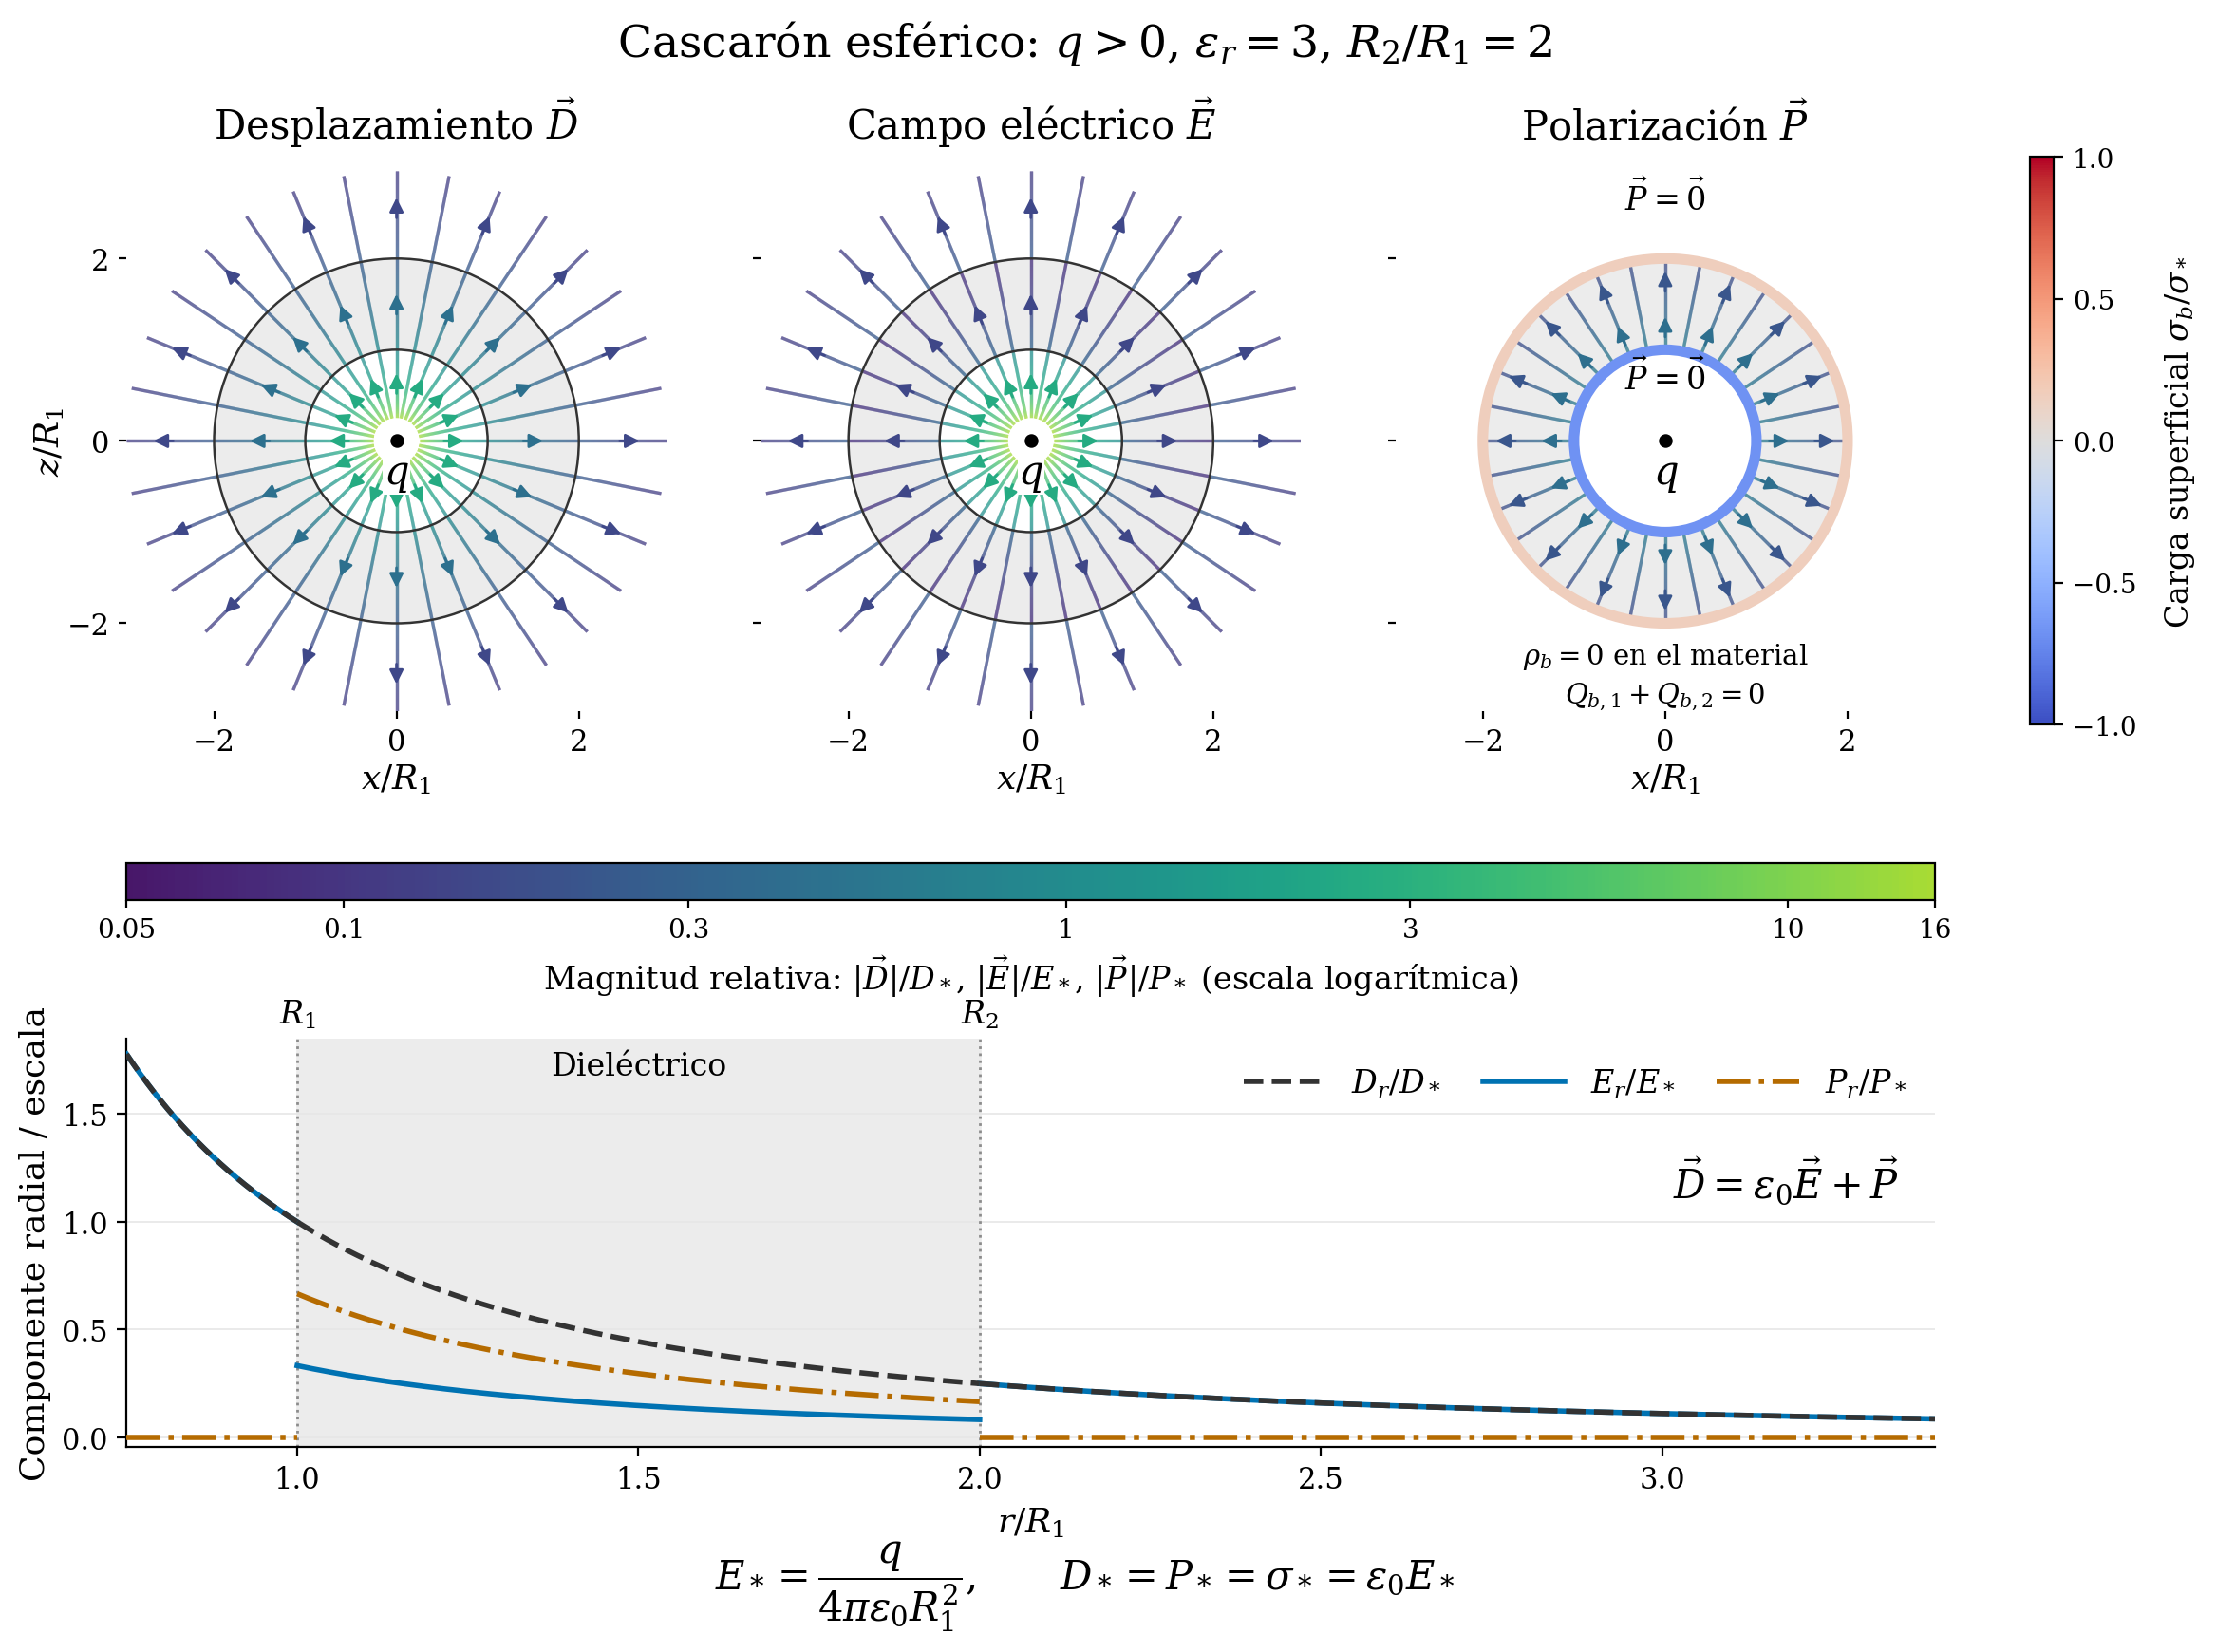
\includegraphics[width=\textwidth]
  {visualizacion_campos_cascaron.png}

\caption{Campos y cargas ligadas en un corte $xz$ del cascarón.
Las líneas indican dirección y sentido; su color, la magnitud
relativa. Las superficies azul y roja representan cargas ligadas
negativas y positivas. Abajo se comparan las componentes radiales.}
\label{fig:campos_cascaron}
\end{figure}
\end{document}
